\section{Reconstructing the linear power from the parameters (version 2)} 
\label{app:linP_approx}

At the end, we coded up our emulator to work in comoving units, i.e., \Mpc.
The main reason was to make it easier to compare different boxes and snapshots,
with the same cosmic variance in the Fourier modes. 
If we had used velocity units in the emulator, different snapshots would have
had different fundamental modes, and different noise at a given wavenumber.
As a consequence, our thermal broadening and pressure smoothing are also
in comoving units, even though they would probably make more sense in velocity
units (temperature sets the thermal broadening scale in velocity units).

My point is that if it was not because the limited box sizes, and limited
number of realisations, we could have coded up the emulator in velocity units.
For instance, this is what was done in \cite{McDonald2005a}.
Given a cosmological model, or a point in a Planck chain, we want to figure
out its linear power spectrum at several redshifts (in velocity units) and
ask the emulator/interpolator to make a prediction for the flux power spectrum
(also in velocity units).

In the rest of this appendix we assume that we have set up the emulator to
work in velocity units. 
We will add at some point text on why the same reasoning would apply when
working in comoving coordinates, but it might be clearer to start with this.


\subsubsection{Velocity units}

We will use $k$ to refer to the (modulus of the) 3D wavenumbers in comoving
coordinates, i.e., in \Mpc. 
We will use $q$ to refer to the save wavenumber in velocity units. 
They are related by:
\begin{equation}
 k = \frac{H(z)}{1+z} ~ q = M(z) ~ q ~.
\end{equation}
$M(z)$ will play an important role in this discussion.

We will use $P(k)$ to refer to (3D) power spectra in comoving units, i.e.,
with units of $\Mpc^3$.
We will use $Q(q)$ to refer to (3D) power spectra in velocity units, i.e.,
with units of $\kms^3$.
They are related by:
\begin{equation}
 Q(z,q) = M^3(z) ~ P(z,k=M(z)q) ~.
\end{equation}


\subsubsection{Linear growth}

At the end we might want to report results at some pivot redshift $z_\ast$,
so it is useful to discuss how the linear power spectrum at $z$ relates to the
linear power spectrum at $z_\ast$.
We ignore neutrinos for now, and assume that we will always care about the 
CDM+baryons power.
In this case we can use the linear growth factor $D(z)$, defined as
\begin{equation}
 P(z,k) = \left[\frac{D(z)}{D_\ast}\right]^2 P_\ast(k) ~,
\end{equation}
where in general functions $y_\ast = y(z_\ast)$.


\subsubsection{Fiducial cosmology}

In our code we will use a fiducial cosmology as a reference, and parameterize
our models as deviations from that cosmology.
We will use either subscripts $_0$ or supperscripts $^0$ to identify functions
for the fiducial cosmology.

We can now define the ratio of the linear power between any model and the
fiducial one, at the central redshift $z_\ast$, and in velocity units:
\begin{equation}
 B(q) = \frac{Q_\ast(q)}{Q^0_\ast(q)} ~.
\end{equation}
This will be another important function, tightly related to the linear
power parameters that we will end up using.


\subsubsection{Putting everything together}

We can now write our desired power spectrum as a function of the fiducial
one, with small corrections that take into account the difference between
the cosmologies:
\begin{align}
 Q(z,q) &= M^3(z) ~ P(z,k=M(z)q)    \\
  &= M^3(z) ~ \left[\frac{D(z)}{D_\ast}\right]^2 P_\ast(k=M(z)q) \nonumber \\
  &= \left[\frac{M(z)}{M_\ast}\right]^3 \left[\frac{D(z)}{D_\ast}\right]^2 
    Q_\ast(q^\prime=M(z)/M_\ast q)    \nonumber \\
  &= \left[\frac{M(z)}{M_\ast}\right]^3 \left[\frac{D(z)}{D_\ast}\right]^2 
    B(q^\prime=M(z)/M_\ast q) ~ Q^0_\ast(q^\prime=M(z)/M_\ast q)  \nonumber \\
  &= \left[\frac{M(z)}{M_\ast}\right]^3 \left[\frac{D(z)}{D_\ast}\right]^2 
    B(q^\prime=M(z)/M_\ast q) \left[ M_\ast^0 \right]^3 
    P^0_\ast(k=M_\ast^0 M(z) / M_\ast q)  \nonumber \\
  &= \left[\frac{M(z)}{M_\ast}\right]^3 \left[\frac{D(z)}{D_\ast}\right]^2 
    B(q^\prime=M(z)/M_\ast q) \left[ M_\ast^0 \right]^3 
    \left[\frac{D^0_\ast}{D_0(z)}\right]^2 
    P^0(z,k=M_\ast^0 M(z) / M_\ast q)  \nonumber \\
  &= \left[\frac{M(z)}{M_\ast}\right]^3 \left[\frac{D(z)}{D_\ast}\right]^2 
    B(q^\prime=M(z)/M_\ast q) \left[ \frac{M_\ast^0}{M_0(z)} \right]^3 
    \left[\frac{D^0_\ast}{D_0(z)}\right]^2 
    Q^0(z,q^\prime= (M_\ast^0 M(z)) / (M_\ast M_0(z)) q)  \nonumber \\
  &= \left[m(z) \right]^3 \left[d(z)\right]^2 
    B(q^\prime=m(z) M_0(z)/M^0_\ast q) ~ Q^0(z,q^\prime=m(z)q) \nonumber ~,
\end{align}
where for convenience we have defined two functions,
\begin{equation}
 m(z) = \frac{M(z)}{M_\ast} \frac{M_\ast^0}{M_0(z)} 
\end{equation}
and 
\begin{equation}
 d(z) = \frac{D(z)}{D_\ast} \frac{D^0_\ast}{D_0(z)} ~,
\end{equation}
that describe differences in expansion rate and in linear growth respectively.

\begin{figure}[ht]
 \begin{center}
  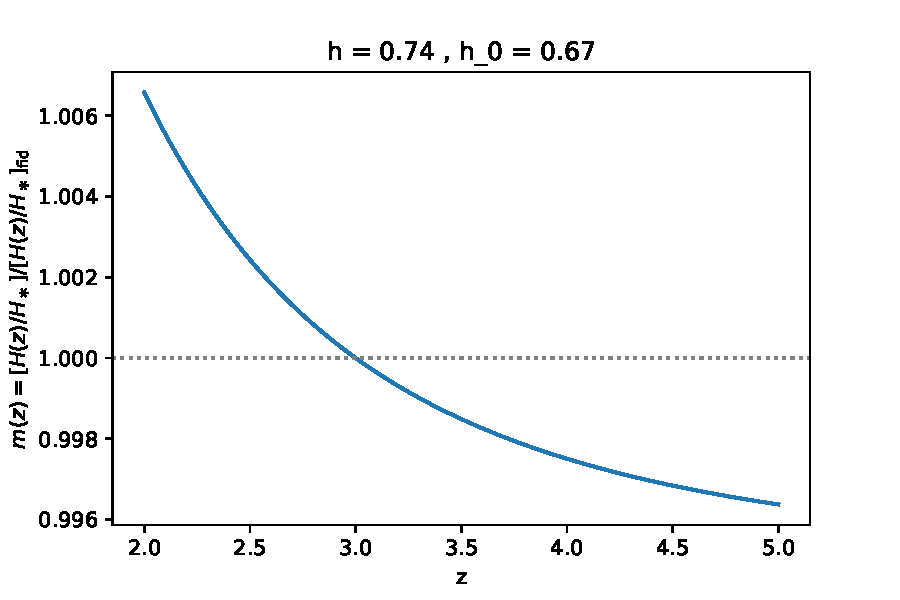
\includegraphics[scale=0.5]{Figures/mz_h074}
  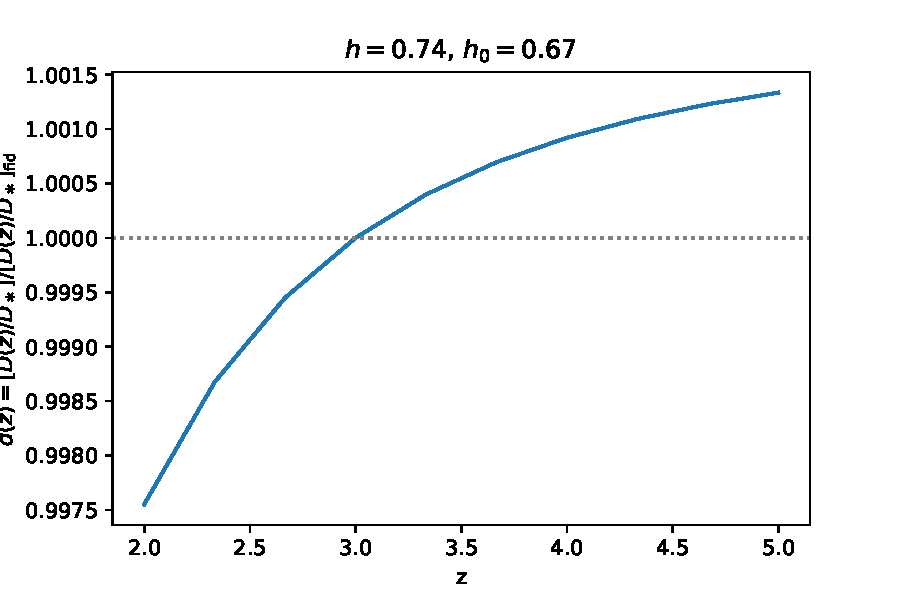
\includegraphics[scale=0.5]{Figures/dz_h074}
 \end{center}
 \caption{Differences in the expansion rate ($m(z)$, left) and in the
  linear growth ($d(z)$,right) with respect to the fiducial cosmology.}
 \label{fig:mz_dz}
\end{figure}

As can be seen in Figure \ref{fig:mz_dz}, even for a model with a very
different value of $H_0$ (and therefore $\Omega_m$) these functions are 
really close to one within the relevant redshift range.
This motivates us to approximate these functions with a parameterized version.
Below we discuss $g_\star$ and $f_\star$ as one-parameter approximations,
but for the main part of the analysis we can just ignore these functions.

If we make the approximation $m(z)=1$ and $d(z)=1$, then we reconstruct
the linear power spectrum with:
\begin{equation}
 Q(z,q) \approx B(q^\prime= M_0(z)/M^0_\ast q) ~ Q^0(z,q) ~.
\end{equation}



